\documentclass[11pt]{article}
\usepackage[T1]{fontenc}
\usepackage{lmodern,microtype}
\usepackage[margin=1in]{geometry}
\usepackage{amsmath,amssymb,amsthm,mathtools}
\usepackage{booktabs,longtable,array}
\usepackage{enumitem,listings,tikz}
\usetikzlibrary{arrows.meta,positioning}
\usepackage{xurl,hyperref}
\hypersetup{hidelinks,pdftitle={Compiled Orbit Transfers and Selective Normal-Disc Witnesses},pdfauthor={ProveIt research continuation}}
\usepackage{fancyhdr}
\pagestyle{fancy}\fancyhf{}
\fancyhead[L]{\small Compiled orbit transfers}
\fancyhead[R]{\small ProveIt research continuation}
\fancyfoot[C]{\thepage}
\setlength{\headheight}{14pt}
\setlength{\emergencystretch}{2em}
\setlist{itemsep=3pt,topsep=5pt}
\newtheorem{theorem}{Theorem}[section]
\newtheorem{lemma}[theorem]{Lemma}
\newtheorem{proposition}[theorem]{Proposition}
\newtheorem{corollary}[theorem]{Corollary}
\theoremstyle{definition}\newtheorem{definition}[theorem]{Definition}
\newtheorem{example}[theorem]{Example}
\theoremstyle{remark}\newtheorem{remark}[theorem]{Remark}
\newcommand{\Z}{\mathbb Z}
\newcommand{\N}{\mathbb N}
\newcommand{\F}{\mathbb F}
\newcommand{\one}{\mathbf 1}
\newcommand{\poly}{\operatorname{poly}}
\newcommand{\supp}{\operatorname{supp}}
\newcommand{\bits}{\operatorname{bits}}
\newcommand{\circuit}{\mathcal C}
\newcommand{\orbits}{\mathcal O}
\newcommand{\Pstate}{\mathcal P}
\newcommand{\commit}{\texttt{b365341b1939c69a26b31bb5d05a097d4572692c}}
\lstset{basicstyle=\small\ttfamily,columns=fullflexible,keepspaces=true,
  breaklines=true,frame=single,showstringspaces=false,tabsize=4}
\title{\textbf{Compiled Orbit Transfers and\\Selective Normal-Disc Witnesses}\\[0.6em]
\large A proof-backed local improvement toward\\quasi-polynomial unknot recognition}
\author{ProveIt research continuation}
\date{October 2026}
\begin{document}
\maketitle
\begin{abstract}
The maintained ProveIt component engine can identify compressing-disc components
of a supplied normal surface using three additive weights. Its full-coordinate
interface instead transports all $7t$ normal coordinates and returns a census of
all component types. We separate these tasks. A source-bound Agol--Hass--Thurston
orbit trace is compiled into a value-independent, nonnegative integer linear
circuit. A few scalar evaluations select an emitted component class; a single
reverse accumulation then recovers one representative's source profile. Interval
ownership converts that profile into its normal coordinates without a
$7t$-dimensional transport pass.

We prove correctness, polynomial encoded size, coefficient-bit bounds, a
selective-extraction theorem, and an explicit family separating selective
extraction from a full dense census: $D+1$ distinct dense profiles require
$\Omega(D^2)$ scalar output entries, whereas one profile is obtained through an
$O(D\log(D+2))$-size circuit. A separate terminal contract certifies an actual
normal compressing disc without trusting the compiler. The stronger claim that
the vector is a component of the original surface is distinguished from this
terminal contract.

The archive includes an executable standard-library implementation, 24 passing
test methods, a 10,000-system literal-graph audit, and controlled measurements.
Sparse eager transport outperforms cold circuit compilation on many fixtures;
on the dense-profile family at $D=1024$, selective extraction is about $3.47$
times faster than that stronger sparse control. These are local interval-query
measurements, not whole-knot timings. The native normal-surface adapter is
source-reviewed but was not executed in this environment. No general
quasi-polynomial recognition bound is claimed: geometric provenance, useful
surface discovery, compressed cutting, and global progress remain separate
obligations.
\end{abstract}
\vspace{0.4em}
\noindent\textbf{Audited repository revision.}\quad\commit.
\par\noindent\textbf{Deliverable policy.}\quad Additive research package; no production dispatch
or repository files were changed.
\clearpage
\setcounter{tocdepth}{1}
\tableofcontents
\vspace{1.3em}
\subsection*{Reading guide}
Sections~\ref{sec:compiler}--\ref{sec:transpose} contain the generic compiler,
size, bit-complexity and selective-extraction proofs.
Sections~\ref{sec:normal}--\ref{sec:certificate} give the normal-disc application
and the independent positive-witness contract.
Section~\ref{sec:separation} establishes the explicit asymptotic separation from
full coordinate censuses. Section~\ref{sec:experiments} records the complete
executed evidence and its limits. Sections~\ref{sec:global}--\ref{sec:questions}
separate the remaining global complexity obligations from the next implementable
research steps.
\clearpage

\section{Research baseline and the precise improvement}
\label{sec:baseline}

\subsection{Read the implementation, not only its status summary}
The relevant baseline is the source at the revision above. The root and synthesis
README files do not summarize every subsequently integrated module. In particular,
sparse component-incidence recovery and weighted component censuses are already
present. Reintroducing either as a new contribution would duplicate completed
work. Our starting points are the maintained files
\path{weighted_orbits.py}, \path{normal_surface_components.py},
\path{normal_component_geometry.py}, and their independent verifiers, together
with \path{synthesis/weighted_components.tex} \cite{repo}.

The component census has a cheap three-weight disc mode and an expensive
$7t$-coordinate mode. Both operate on a supplied normal vector, not on a search
space of vectors. The latter is useful when a subsequent operation needs a
specific geometric surface rather than just a count. That transition---from
recognizing a good component to retrieving it---is the target of this report.

Classical weighted orbit counting and normal-component extraction are already
polynomial in their encoded input parameters \cite[Theorem 16 and Corollary 17]{aht}.
The improvement here is therefore not a new polynomial-time orbit algorithm.
It is a more selective interface and a different organization of the arithmetic:
retain a shared linear computation, identify a useful output with a small payload,
and recover only the coordinates actually requested.

\subsection{Contribution ledger}
The mathematical and experimental claims have different status.
\begin{center}
\begin{tabular}{p{0.29\textwidth}p{0.61\textwidth}}
\toprule
Item & Status and scope\\
\midrule
Orbit-transfer circuit & Proved and implemented for complete, locally checked
interval traces. No represented-point expansion.\\[0.3em]
Selected source profile & Proved and implemented by exact reverse accumulation.
One output uses seed $1$, not its multiplicity.\\[0.3em]
Normal-disc extraction & Proved assuming the validated native arc/ownership
encoding; a source-reviewed adapter is supplied. Native execution is pending.\\[0.3em]
Independent positive witness & A precise contract and native-verifier bridge are
supplied. It verifies a disc, not component membership in the original vector.\\[0.3em]
Performance & Executed local-query comparisons against both dense and sparse
eager controls; gains and regressions are retained.\\[0.3em]
General recognition & No new unconditional quasi-polynomial bound and no
whole-knot speedup established by this package.\\
\bottomrule
\end{tabular}
\end{center}

\subsection{What is new here, and what is not}
Weighted AHT transfer is the underlying geometric-combinatorial operation. The
transposition of a linear program is also a standard technique; modern
formalizations explicitly separate linearization from cost-preserving
transposition \cite{radul}. We do not claim to originate either idea. The
contribution is their concrete combination in this code path: a
\emph{value-independent interval compiler}, a proof that its intermediate and
reverse coefficients remain small in bits, a sparse normal-coordinate ownership
interface, and a terminal verifier contract that does not enlarge the trusted
compiler boundary. The dense-profile family makes the avoided output cost exact.
No claim of exhaustive literature priority is made.

\section{Encoded orbit systems and source-bound traces}
\label{sec:model}

\subsection{Intervals, pairings, and source atoms}
Fix the integer universe $X_N=\{0,\ldots,N-1\}$. An interval pairing is an
order-preserving or order-reversing bijection between two equally long integer
intervals. The equivalence relation generated by all pairings partitions $X_N$
into orbits. The integer $N$ and all endpoints are binary encoded; an algorithm
that scans $N$ points is not an encoded polynomial-time algorithm.

The public native trace uses inclusive rows $(a,b,c,d,\epsilon)$ with
$\epsilon\in\{1,-1\}$, $a\le c$, and $b-a=d-c$. It identifies $x$ with
$x+c-a$ when $\epsilon=1$, and with $a+d-x$ when $\epsilon=-1$.
In contrast, source weight and ownership intervals in this report are half open.
The conversion $[a,b]\leftrightarrow[a,b+1)$ is explicit throughout.

Choose a source partition
\[
 0=s_0<s_1<\cdots<s_m=N,\qquad I_j=[s_{j-1},s_j),\quad 1\le j\le m.
\]
The partition must include \emph{all} endpoints used by both the cheap decision
weights and the eventual coordinate-ownership queries. It is fixed before
compilation. Let $z_j$ be a formal variable denoting the constant scalar value at
each point of $I_j$. For an original orbit $O$, define its source profile
\begin{equation}
 \lambda(O)_j=|O\cap I_j|,\qquad
 L_O(z)=\sum_{j=1}^m\lambda(O)_jz_j.
 \label{eq:profile}
\end{equation}
A leaf variable is a \emph{per-point value}, not the total weight of its interval.
Consequently reverse accumulation returns counts $\lambda(O)_j$ directly; one
must not multiply them by $|I_j|$ again.

\subsection{The proof boundary}
A trace contains the initial universe and ordered canonical pairing list, an
orbit count, and a complete sequence of local operations. The supplied checker
validates identity deletion, static contraction, reflection trimming, periodic
merging, transmission by powers of a partial inverse, and suffix truncation.
It checks source equality and requires the final universe and pairing list to
be empty. A valid prefix is not a certificate of an orbit count.

The checker is an attributed adaptation of the maintained MIT-0 local verifier,
not a byte-identical upstream snapshot. It does not invoke the reference
scheduler. Both the classical merger convention and the maintained sharp
periodic-merger convention are accepted when their respective local inequalities
hold. Soundness of a supplied trace does not require it to follow the producer's
preferred schedule. A polynomial bound in \emph{source input alone}, however,
requires a polynomial-length schedule. Our unconditional compilation bound is
in the explicit supplied trace; classical AHT scheduling supplies the standard
polynomial trace-size guarantee \cite{aht}.

Only two kinds of accepted events alter weights: deleting a suffix while
transferring its weight to surviving points, and contracting static intervals
while emitting their orbit weights. The other operations change the presentation
of the same current equivalence relation without changing its point set or
point weights. The compiler consumes the checked weight-moving events rather
than performing a second orbit search.

\begin{remark}[No hidden topological assertion]
A checked trace asserts a statement about interval equivalence classes. It does
not establish that the input is the arc system of a surface, that a supplied
triangulation is a knot exterior, or that a normal surface was found by a complete
search. Those assertions require additional, source-bound constructions.
\end{remark}

\subsection{A latent partition invariant}
For the proofs, associate to each surviving current point $x$ a nonempty set
$B_x$ of original points. These sets are pairwise disjoint. Together with already
emitted original orbits, they partition $X_N$. Initially $B_x=\{x\}$. When a
suffix point is mapped to an earlier representative, its set is unioned into
that representative's set. A static current point corresponds to one complete
original orbit and is then emitted.

The maintained weight at $x$ is the formal linear expression
\[
 W_x(z)=\sum_{j=1}^m |B_x\cap I_j|z_j.
\]
The sets $B_x$ are a proof device, never an explicit data structure. Their
nonemptiness and disjointness are important: they yield bit bounds for both
forward circuit values and reverse coefficients.

\section{Compiling a monotone transfer circuit}
\label{sec:compiler}

\subsection{Circuit language and interval runs}
The circuit has zero, input, addition, and nonnegative-integer scaling nodes:
\[
 0,\qquad z_j,\qquad u+v,\qquad q u\quad(q\in\N).
\]
Input values may be signed; the \emph{coefficients of the linear program} are
nonnegative. Each current interval run carries a circuit-node identifier whose
formal value is its per-point profile expression. At initialization, $I_j$
carries $z_j$. Two adjacent runs may be merged when their node identifiers are
equal. No equality test on one numerical evaluation may justify a structural
merge.

The implementation shares nodes by exact keys, simplifies zero additions and
unit scalings, and replaces $u+u$ with $2u$. This sharing is an optimization, not
a mathematical assumption. Disabling it would retain the polynomial construction
bound, with repeated nodes counted separately.

\subsection{Translation suffixes}
Suppose a checked translation truncation changes the current universe from
$[0,n)$ to $[0,c)$ and the carrier has positive period $p$. Its local conditions
ensure $b=c-p\ge0$. Each removed point has surviving representative
\begin{equation}
 \rho(x)=b+((x-b)\bmod p),\qquad x\in[c,n).
 \label{eq:fold}
\end{equation}
Indeed, repeated inverse translation decreases $x$ by $p$ until it first falls
below $c$, landing in $[c-p,c)$. Every intermediate inverse is defined by the
truncation contract.

Consider the removed part $[\ell,h)$ of one run carrying expression $u$. Write
\[
 h-\ell=qp+r,\qquad 0\le r<p,
 \quad a=b+((\ell-b)\bmod p).
\]
It contributes $qu$ on $[b,c)$ and one extra $u$ on the cyclic interval of
length $r$ beginning at $a$. The latter is represented by at most two ordinary
intervals. Existing prefix weights are retained.

\begin{lemma}[Quotient transfer]
The above at-most-three interval contributions give exactly the pushforward of
$u$ on $[\ell,h)$ through \eqref{eq:fold}. The construction uses a single binary
quotient and remainder, not $q$ iterations.
\end{lemma}
\begin{proof}
Every consecutive block of $p$ integers meets each residue modulo $p$ exactly
once. There are $q$ such complete blocks and one residual block of length $r$.
Its residues occur consecutively on the residue circle, crossing its chosen cut
at most once. Each target point therefore receives either $q$ or $q+1$ copies
of the source expression, with the extra copy on precisely the residual arc.
\end{proof}

\subsection{Reflection suffixes and static contractions}
For a checked trimmed reflection, the carrier has map $x\mapsto a+n-1-x$.
The deleted part $[\ell,h)$ of a run maps to
\begin{equation}
 [a+n-h,\ a+n-\ell).
 \label{eq:reflection}
\end{equation}
Trimming ensures the image lies in the surviving prefix. The coefficient is
one, and the interval orientation has no further effect on an additive weight.

For a static contraction, split current runs at the endpoints of all deleted
gaps. A run piece of length $\mu$ with expression $u$ inside a static gap emits
an ordered record $(u,\mu)$. It stands for $\mu$ distinct original orbits with
that same formal profile. Surviving pieces are shifted by the exact total length
of preceding deleted gaps. The count $\mu$ remains binary encoded.

\subsection{Why a numerical difference sweep is not the compiler}
A conventional weighted implementation accumulates signed endpoint differences
and updates a numerical vector while sweeping. This is perfectly appropriate
for a fixed query. Directly turning that procedure into a symbolic expression
would introduce subtraction and could make the size of intermediate reverse
coefficients harder to control. More importantly, numerical equality between
neighbouring runs would erase distinctions needed by a later ownership query.

Our compiler uses an active-contribution tree. Each contributed interval has a
temporary leaf containing either its expression or zero according to whether it
is active. Internal tree nodes add their children. Changing one leaf creates at
most logarithmically many new arithmetic nodes. The tree array itself is mutable;
previously created arithmetic nodes remain immutable in the circuit.
At an endpoint, intervals that end are removed \emph{before} intervals that
begin are added. Thus intermediate active sets are subcollections of the valid
left or right active set. A run's output expression is the tree root after the
endpoint updates.

This is a persistent arithmetic computation, not a persistent point set. It
supports enormous intervals with a finite collection of endpoints, quotient
coefficients, and expression identifiers.

\begin{lemma}[Value independence]
For a fixed checked trace and source partition, the emitted circuit records are
independent of the numerical values subsequently assigned to $z_1,\ldots,z_m$.
They evaluate correctly for every integer assignment, including signed ones.
\end{lemma}
\begin{proof}
Initial leaves depend only on the source partition. Every later branch depends
on interval endpoints, a trace event, an integer quotient/remainder, a zero node,
or exact node identity. None depends on an evaluated query. The transfer formulas
are linear identities, valid for arbitrary integer values, and addition-tree
updates combine precisely the active contributions. Induction over the accepted
trace proves the claim.
\end{proof}

\begin{theorem}[Transfer representation]
\label{thm:representation}
Let a complete source-bound trace have $C$ original orbits. The compiler emits
records $(u_e,\mu_e)$ such that the original orbits can be partitioned into
classes $\orbits_e$ satisfying
\[
 |\orbits_e|=\mu_e,\qquad
 u_e(z)=L_O(z)\quad\text{for every }O\in\orbits_e,
 \qquad \sum_e\mu_e=C.
\]
Every original orbit appears in exactly one emitted class. Classes with the
same profile need not have been merged.
\end{theorem}
\begin{proof}
Maintain the latent partition invariant from Section~\ref{sec:model}. On each
current run, its circuit expression gives the source profile of every latent
set $B_x$ there. This is true for singleton initial sets. Equivalence-preserving
presentation changes do not affect it. Translation and reflection pushforwards
union the latent sets of removed points into surviving representatives, and
the preceding interval formulas give their profile sums. Disjointness is
preserved because each removed point has exactly one surviving image.

When a static gap is contracted, each of its current points is an isolated orbit
of the current relation. Its latent set is therefore one complete original
orbit. Every point in a run piece has the same profile expression, so emitting
its length as a multiplicity is correct. Completeness of the trace leaves no
surviving point, and the latent partition exhausts $X_N$. This proves both the
representation and the multiplicity identity.
\end{proof}

\section{Size bounds and exact bit complexity}
\label{sec:cost}

\subsection{A breakpoint bound that does not use numerical coincidences}
Let $L$ be the number of explicit trace records, $F$ the number of suffix
truncations, and $G$ the sum of the numbers of static gap intervals in all
contraction records. Define the conservative bound
\begin{equation}
 R=m+4F+2G.
 \label{eq:R}
\end{equation}
The bound concerns stored geometric runs, including redundant boundaries between
formally equal expressions. It does not presume an expensive symbolic equality
test.

\begin{lemma}[Run growth]
\label{lem:runs}
The compiler has at most $R$ current runs at every stage. A contraction with $g$
gaps emits at most the current number of runs plus $2g$ pieces. Consequently the
total number $E$ of emission records is $O(LR+G)$.
\end{lemma}
\begin{proof}
During a translation fold, surviving-prefix breakpoints remain. A breakpoint
strictly within the deleted suffix contributes at most one new breakpoint after
reduction modulo $p$. Neighbouring old runs share a boundary, so its two
appearances in the piece descriptions yield the same residue endpoint, not two
unrelated cuts. Endpoints introduced by cutting a straddling run and by choosing
the residue interval are among a constant number of extra boundaries. Four is
a safe allowance. A reflection sends each suffix breakpoint to one reflected
breakpoint, again with at most a constant number of new outer boundaries.

For contraction, adding endpoints of $g$ gaps makes at most $2g$ extra pieces.
Deleting gap pieces and shifting the rest does not create any further boundary.
Summing these bounds proves \eqref{eq:R}. Emissions are among the split pieces
at contractions; summing over at most $L$ records gives the stated bound.
\end{proof}

This is the symbolic version of the breakpoint accounting behind weighted AHT
transfer. The crucial point is that it applies before evaluating the formal
variables. A leaf for every original point would violate the encoded model; a
leaf for every source \emph{interval} does not.

\begin{theorem}[Compilation size]
\label{thm:size}
Let $V$ denote the cost of independently checking the supplied trace. A circuit
with
\begin{equation}
 K=O\bigl(1+m+FR\log(R+2)\bigr)
 \label{eq:K}
\end{equation}
zero/input/arithmetic nodes can be compiled, with $E=O(LR+G)$ emissions.
Apart from $V$, compilation uses
$\widetilde O(m+LR+G)$ endpoint and exact-integer operations. Its encoded running
time and storage are polynomial in the explicit input, trace, and source
partition. Under a polynomial-length AHT schedule they are polynomial in the
usual encoded orbit input parameters.
\end{theorem}
\begin{proof}
Each old run supplies at most four pieces at a fold: a retained-prefix piece,
a whole-period multiple, and two remainder pieces. There are $O(R)$ pieces,
$O(R)$ endpoint updates, and $O(\log(R+2))$ tree nodes per update. A whole-period
contribution creates at most one scaling node. Summing over $F$ folds gives
\eqref{eq:K}. Contractions only split, emit, and shift expression identifiers;
they require no new arithmetic nodes. Sorting endpoints and scanning the
resulting pieces gives the remaining bound. The tilde suppresses logarithmic
factors from sorting, indexing, and dictionaries.

The implementation uses exact-key hash tables. Its size bound is deterministic;
the usual expected hash-table operation cost is used in the implementation-level
time estimate. Replacing these tables with comparison dictionaries introduces
additional logarithmic factors but preserves deterministic polynomial encoded
complexity. Nothing in the size proof expands the universe or iterates an encoded
quotient.
\end{proof}

\subsection{Intermediate coefficients stay small in bits}
Put $B=\lceil\log_2(N+1)\rceil$. For a circuit node $v$, write its formal
coefficient vector as $a_v\in\N^m$.

\begin{lemma}[Mass bound]
\label{lem:mass}
Every nonzero circuit node satisfies
\[
 1\le\|a_v\|_1\le N.
\]
Every scaling coefficient is at most $N$. If input values satisfy $|z_j|\le W$,
then every forward value has absolute value at most $NW$.
\end{lemma}
\begin{proof}
Actual run nodes describe a nonempty latent set and hence have mass at most
$N$. A quotient-scaled contribution describes a subcollection of the latent sets
mapping to one residue representative, so the same bound holds. Internal
addition-tree nodes describe subcollections of active contributions to a target.
At a boundary, removing ending pieces before adding starting pieces ensures that
transient subcollections remain subsets of the valid collection on one side.
Thus no transient gate counts an original point twice. Initial leaves have mass
one. Scaling quotients cannot exceed the number of current points, and evaluation
at bounded signed values obeys the triangle inequality.
\end{proof}

The argument also explains the choice of a monotone compiler. With arbitrary
cancellation gates, small final coefficients alone would not bound intermediate
ones. Here nonnegativity supplies that control at the representation level.

\subsection{Bit accounting}
Forward payload arithmetic uses $O(B+\log(W+1))$-bit integers. Endpoint arithmetic
and quotients use $O(B)$ bits. Node identifiers use $O(\log(K+2))$ bits. It is
therefore valid to replace each arithmetic operation in the preceding bounds
by an explicit polynomial bit cost, for example grade-school integer arithmetic;
one must not treat a huge quotient as a unit-cost unbounded machine integer.

The checker additionally reads the explicit integers occurring in the trace.
An adversarial trace may contain unnecessarily long records or huge encoded
powers; its own encoded length is included in $V$. A source polynomial-time
claim is justified only for a source-polynomial-size produced trace, not for
arbitrary redundant supplied evidence.

Retaining the circuit uses $O(K(B+\log(K+2)))$ bits for the coarse gate encoding,
plus the current runs, source cuts, emissions and supplied proof. This may be
larger than an eager computation's current working state. The time improvement
is not a claim of uniformly lower memory.

\section{Selective extraction by one transpose}
\label{sec:transpose}

\subsection{Reverse accumulation}
To recover the profile of an emission $u_e$, seed its adjoint by $1$. Process
nodes in reverse topological order. At $v=u+w$, add the adjoint of $v$ to those
of $u$ and $w$. At $v=qu$, add $q$ times the adjoint of $v$ to that of $u$.
The resulting adjoints at the input leaves are the coefficients of $u_e$.

\begin{theorem}[Selective source-profile extraction]
\label{thm:transpose}
For an emission $e$, one reverse traversal returns exactly $\lambda(O)$ for
any $O\in\orbits_e$. It uses $O(K)$ exact-integer operations. Every nonzero
intermediate adjoint in this single-output traversal is at most $N$.
\end{theorem}
\begin{proof}
The reverse rules are the coefficient identities for addition and scalar
multiplication. Induction down the acyclic graph therefore computes the
coefficient of each input in $u_e$, which is the desired profile by
Theorem~\ref{thm:representation}.

For the adjoint bound, the final coefficient of a nonzero node $v$ in the output
expression is a nonnegative integer $\alpha_v$. Expanding the circuit and
collecting paths through $v$ gives a contribution $\alpha_v a_v$ to the output's
nonnegative coefficient vector. Hence
$\alpha_v\|a_v\|_1\le\|a_{u_e}\|_1\le N$.
During reverse accumulation only nonnegative partial contributions are added,
so every intermediate adjoint is bounded by its final value. Lemma~\ref{lem:mass}
gives $\|a_v\|_1\ge1$. The distinguished zero node need not be traversed.
\end{proof}

\begin{corollary}[Cheap selection followed by one witness]
Suppose a predicate of $d$ scalar orbit sums identifies an acceptable emission.
After compilation, $d$ forward passes, a scan of the $E$ emissions, and one
reverse pass select and recover a profile in
\[
 O((d+1)K+dE+m)
\]
arithmetic operations, apart from preparing the scalar inputs. The predicate
need not be linear: only its $d$ input statistics must be linear.
\end{corollary}

\subsection{Interval ownership avoids a dense incidence matrix}
A coordinate query is an additive list of ownership records
$(q,\ell,h)$ with endpoints in the source partition. Each original point in
$[\ell,h)$ contributes one to coordinate $q$. Let there be $Q$ records and $D$
output coordinates. For a selected profile $\lambda$, compute the prefix sums
\[
 P_0=0,\qquad P_j=\lambda_1+\cdots+\lambda_j.
\]
An ownership interval $[s_a,s_b)$ contributes $P_b-P_a$. Multiple intervals
for the same coordinate are added; overlapping ownership records are allowed
and have their stated additive meaning.

\begin{theorem}[Selective coordinate extraction]
\label{thm:ownership}
After the selected transpose, all $D$ coordinates can be recovered using
$O(m+Q+D)$ integer additions and subtractions when endpoint indices are supplied.
The bundled API finds endpoint indices by binary search and therefore performs
an additional $O(Q\log(m+2))$ endpoint comparisons. No $D\times m$ incidence
matrix or $D$-dimensional forward payload is formed.
\end{theorem}
\begin{proof}
For each ownership interval, its contribution is exactly the sum of the profile
entries for source atoms inside the interval. The prefix-difference formula
computes this sum in two accesses and one subtraction. The initial prefix pass
and final coordinate array have the stated sizes. The source partition validation
ensures there is no partially cut atom.
\end{proof}

\subsection{Multiplicity and reuse boundaries}
If the objective is one component, the seed is $1$. Seeding by $\mu_e$ instead
returns the sum of the profiles of all $\mu_e$ components in that emitted class.
Both are useful operations, but they have different meanings. A static universe
with no pairings illustrates the difference: one emission may have multiplicity
$N$ and profile $(1)$, whereas the aggregate profile is $(N)$.

For $q$ individually requested emissions, independent reverse traversals cost
$O(qK)$. A single traversal with several weighted seeds returns an aggregate,
not $q$ separated profiles. Arbitrary signed seed combinations require charging
the seed bit lengths as well; the $N$ adjoint bound above is a single-output
statement. These observations do not supply a free full census.
Similarly, changing only numerical weights on the same source partition permits
reuse, but adding new endpoints requires refinement and recompilation. Changing
the relation, normal vector, or triangulation invalidates the old source binding.

\begin{example}[A numerical merge that loses a witness]
Take two isolated points with separate source atoms. A cheap weight assigning
zero to both produces a one-row numerical histogram of multiplicity two. The
ownership profiles remain $(1,0)$ and $(0,1)$. Treating the equal numerical values
as one reusable symbolic state cannot recover both correctly. The compiler
retains their distinct source expressions even though the cheap histogram may
subsequently group their evaluated values.
\end{example}

\section{Application to normal compressing discs}
\label{sec:normal}

\subsection{Geometric contract}
Let $M$ be a compact connected orientable triangulated 3-manifold with one torus
boundary, and let $x\in\N^{7t}$ be an admissible normal vector. Admissibility
includes matching equations and the quadrilateral constraints. Assume the
validated native construction supplies an arc-equivalence system with one orbit
per connected component of the represented surface.

The native ownership construction chooses one corner on each normal polygon.
For each nonzero polygon type its chosen corners form one consecutive interval
in an oriented global-edge block. Thus its coordinate is an interval ownership
sum. At most four triangle types and one quadrilateral type are nonzero in each
tetrahedron, so there are at most $5t$ such ownership intervals. Zero coordinates
are still present in the final $7t$-vector. All edge blocks and interval lengths
are binary encoded; an enormous number of normal polygons does not imply an
enormous ownership list.

The following application uses that native geometric contract. This report's
standalone graph tests do not replace the existing manifold and normal-surface
validator, nor do they independently re-establish its source encoding.

\subsection{Three statistics are enough to choose a disc}
For each component $S$, the native three-weight system computes
\[
 \chi(S),\qquad h_1(S),\qquad h_2(S),
\]
where the last two values are integral intersection counts whose parities give
the boundary class against a homology basis of the boundary torus. Integral
Euler weights assign one credit per vertex, one debit per arc and one credit
per polygon, with each charge owned by a point in its component. The existing
implementation independently checks the proposed boundary basis and the
weighted replay \cite{repo}.

\begin{proposition}[Disc predicate]
\label{prop:disc}
A compact connected component $S$ is a compressing disc for the torus boundary
exactly when
\begin{equation}
 \chi(S)=1,\qquad (h_1(S),h_2(S))\not\equiv(0,0)\pmod2.
 \label{eq:disc}
\end{equation}
\end{proposition}
\begin{proof}
Nonzero boundary homology implies that $S$ has nonempty boundary. By the
classification of compact connected surfaces, an orientable surface has
$\chi=2-2g-b$, and a nonorientable one has $\chi=2-k-b$ with $k\ge1$.
With $b\ge1$, the equation $\chi=1$ forces $g=0,b=1$ in the orientable case
and is impossible in the nonorientable case. Thus $S$ is a disc. Its boundary is
an embedded circle on a torus. An essential such circle has primitive integral
slope and therefore nonzero mod-two homology, while an inessential one has zero
class. This proves both directions. The nonzero-boundary test excludes a closed
projective plane, so no irreducibility hypothesis is needed for this predicate.
\end{proof}

The predicate is applied per component, not to aggregate Euler characteristic
or aggregate boundary parity. For example, the boundary parities of two parallel
meridian discs cancel in total. Aggregate cancellation cannot justify rejecting
the individual discs.

\subsection{The extraction theorem}
\begin{theorem}[One normal-disc vector without a full-coordinate transport]
\label{thm:normal}
Under the geometric contract above, compile a checked arc-system trace using a
partition containing the endpoints of its three decision-weight lists and all
normal-coordinate ownership intervals. If the surface contains a compressing
disc, three forward circuit evaluations and one selected transpose recover the
$7t$-coordinate vector $y$ of an actual such connected component. In particular,
$0\le y\le x$, $y$ is admissible, and the represented surface is a connected
essential disc.

After compilation, the arithmetic cost is
$O(K+E+m+t)$, with an additional $O(t\log(m+2))$ endpoint-comparison overhead in
the supplied API. This does not include the subsequent independent terminal
check.
\end{theorem}
\begin{proof}
By Theorem~\ref{thm:representation}, every component appears in some emitted
class. Three evaluations compute its exact statistics, so
Proposition~\ref{prop:disc} selects an emission precisely when it represents
compressing discs. The transpose recovers the selected class's common source
profile. Each polygon contributes exactly one chosen corner to its own normal
coordinate, so the ownership sums are exactly the component's normal vector.
The native correspondence between arc orbits and components gives the stronger
component claim. The cost follows from the preceding extraction theorems with
$d=3$, $D=7t$, and $Q\le5t$.
\end{proof}

The theorem changes the route to $y$, not the topology it represents. It does not
assume orientability of the selected surface in advance, perform a global
normal-surface search, or infer that the ambient manifold is a knot exterior.

\begin{center}
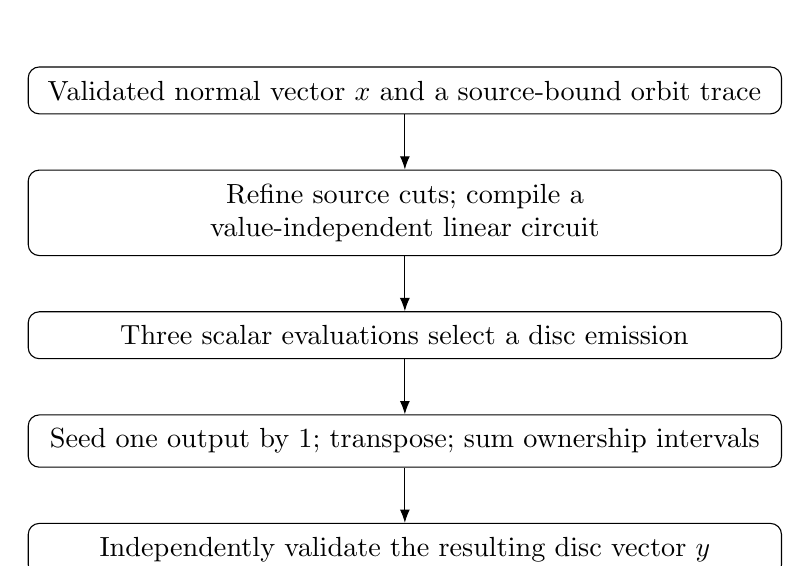
\begin{tikzpicture}[node distance=7mm,box/.style={draw,rounded corners,align=center,
  text width=0.76\textwidth,inner sep=5pt},>=Latex]
\node[box] (source) {Validated normal vector $x$ and a source-bound orbit trace};
\node[box,below=of source] (compile) {Refine source cuts; compile a value-independent linear circuit};
\node[box,below=of compile] (select) {Three scalar evaluations select a disc emission};
\node[box,below=of select] (reverse) {Seed one output by $1$; transpose; sum ownership intervals};
\node[box,below=of reverse] (check) {Independently validate the resulting disc vector $y$};
\draw[->] (source)--(compile);\draw[->] (compile)--(select);
\draw[->] (select)--(reverse);\draw[->] (reverse)--(check);
\end{tikzpicture}
\end{center}

\section{A verifier contract that does not trust the compiler}
\label{sec:certificate}

\subsection{Verify the useful conclusion independently}
A compiler bug must not manufacture a knot verdict. The positive terminal
certificate contains the original source fingerprint, a proposed normal vector
$y$, and an independent native three-weight census certificate for $y$ itself.
The verifier reconstructs the original source, validates $y$ in the same
triangulation, checks $0\le y\le x$, and independently checks that $y$ has exactly
one component and exactly one compressing-disc component. It reads these counts
from the \emph{verified certificate summary}, not from a separately mutable
result wrapper.

This terminal checker does not call the transfer compiler, reverse accumulation,
or coordinate-ownership extraction. Its trust dependencies are the existing
validated geometric encoding, the native independent weighted verifier, and
exact arithmetic. The proof object is about the ambient manifold and vector;
relating that manifold to a diagram still requires a separate provenance
certificate.

\begin{proposition}[Positive terminal soundness]
If the terminal checks above accept, the proposed vector represents one properly
embedded compressing disc in the validated ambient manifold. This conclusion
holds even if the discovery compiler is arbitrarily incorrect.
\end{proposition}
\begin{proof}
The independent geometric validation establishes an admissible embedded normal
surface represented by $y$. The independently replayed census establishes its
connectedness and the disc predicate. Proposition~\ref{prop:disc} therefore
establishes the conclusion. No fact about the computation that proposed $y$ is
used.
\end{proof}

\subsection{Do not overstate what the terminal certificate proves}
The coordinate inequality $y\le x$ does not, by itself, establish that the normal
surface for $y$ is a connected component of the normal surface for $x$.
Compatible normal vectors may sum by a normal-sum operation without their
individual surfaces being disjoint components of the sum. We therefore do not
advertise the positive terminal format as an independent component-membership
certificate. Component membership is a theorem about a correct compiler applied
to the correct native arc system. The terminal independently certifies the
weaker conclusion sufficient for a disc witness.

Likewise, a positive disc in an arbitrary supplied torus-boundary manifold is
not by itself a certificate that an unrelated input diagram is an unknot. The
missing correspondence cannot be replaced by trusting a filename, an invariant
match, or a cached summary.

\subsection{A negative precheck protects the fast path}
For integration, the proposed adapter first runs the maintained three-weight
census on $x$ and independently verifies it. If no disc is present, it returns
\texttt{NO\_DISC\_IN\_SUPPLIED\_VECTOR}; it does not compile a fine ownership
partition. A positive precheck supplies an unweighted trace for compilation.
After extraction, a fresh cheap census on $y$ supplies the terminal certificate.
This costs extra constant-dimensional work on positive instances but avoids
symbolic overhead on negative ones. The standalone timing comparison in
Section~\ref{sec:experiments} does \emph{not} include this geometric adapter.

\subsection{Budgets and interruptions}
The adapter uses one orbit-cycle allowance across the initial and terminal
native censuses, and a separate circuit-node allowance for compilation.
Exhaustion yields \texttt{INCONCLUSIVE}, without publishing an unverified
positive witness. A cooperative callback applies during source validation,
trace checking, compilation, forward and reverse evaluation, extraction, and
independent replay. Callback exceptions propagate, including for callable
objects whose Boolean value is false.

These are cooperative work allowances, not a hostile-input process sandbox.
Large explicit certificates, ownership arrays, and Python integer allocations
must still be bounded by the host. The circuit-node allowance is not silently
presented as an elapsed-time or memory limit on every stage. Invalid options
are rejected before starting geometric work.

\section{An exact asymptotic separation from full censuses}
\label{sec:separation}

It is useful to prove a family where the avoided work is necessary for the old
\emph{output interface}, rather than infer an asymptotic claim from timing plots.
The following construction also tests symbolic sharing after profiles become
dense.

\begin{theorem}[Dense-profile family]
\label{thm:family}
Let $D\ge2$, $p>D$, and $Q\ge1$ be integers. Set
\[
 \ell=Qp+1,\qquad N=D\ell,
\]
and use the single translation pairing $x\sim x+p$ for $0\le x<N-p$.
Partition the source into $D$ consecutive intervals of length $\ell$, each owning
one coordinate. The complete coordinate histogram consists of
\begin{equation}
 Q\one+e_0,\ldots,Q\one+e_{D-1}
 \quad\text{with multiplicity }1\text{ each},\qquad
 Q\one\quad\text{with multiplicity }p-D.
 \label{eq:densefamily}
\end{equation}
In particular, a full explicit sparse-or-dense coordinate histogram has
$\Omega(D^2)$ nonzero scalar entries. Nevertheless, one selected profile can be
extracted using an $O(D\log(D+2))$-size compiled circuit and $O(D\log(D+2))$
arithmetic operations. The bit complexity additionally charges the binary
lengths of $p$ and $Q$.
\end{theorem}
\begin{proof}
The orbits are residue classes modulo $p$. Interval $j$ begins at $j\ell$, whose
residue is $j$, since $j<D<p$. Its length $Qp+1$ gives $Q$ occurrences of every
residue and one extra occurrence of residue $j$. Therefore residue $r<D$ has
profile $Q\one+e_r$, and every remaining residue has profile $Q\one$. All profiles
are distinct and have $D$ positive coordinates, proving the output lower bound.

A single translation truncation reduces the universe to one period and a static
contraction emits all residue representatives. There are $O(D)$ source runs and
$O(D)$ contribution endpoints. The active-contribution tree uses
$O(D\log(D+2))$ gates. Its common full-period contributions share the dense
background $Q\sum_j z_j$, while unit remainders distinguish the exceptional
residues. A singleton marker on the original point $0$, added to the source
partition, identifies residue zero using one scalar query; it introduces only
one additional source cut. The selected transpose and $D$ interval sums obey the
same asymptotic bound. No loop has $p$ or $Q$ iterations.
\end{proof}

This is a lower bound on materializing the \emph{entire histogram}, not on the
intrinsic complexity of retrieving one component. Another selective method may
match or improve the bound. The theorem establishes exactly why an interface
that insists on all component coordinates can do asymptotically unnecessary
work. It does not assert that this family has been realized as the normal arc
systems of knot exteriors.

\subsection{Why sparse vectors alone do not remove this family}
Sparse eager transport is an important control and often a better implementation
choice. It skips absent coordinates and can exploit inexpensive current states.
In \eqref{eq:densefamily}, however, every final profile has every coordinate
present. A full sparse histogram must still materialize $D(D+1)$ positive entries.
The circuit instead shares an expression for the common dense contribution and
transposes only one requested output. This distinguishes \emph{sparse numerical
vectors} from \emph{shared symbolic computations}.

\subsection{Why cold compilation can still lose}
For a tiny query, allocating circuit nodes and an active tree costs more than
updating a short integer vector. If profiles remain sparse, numerical dictionary
updates can be cheaper than preserving a reusable expression history. Also,
a cheap numeric query may coalesce many runs that a universal circuit must keep
separate. Theorem~\ref{thm:family} supplies a genuine asymptotic separation, not a
universal constant-factor improvement. Dispatch should be based on measured
payload growth and reuse needs, not on the existence of a theorem alone.

\section{Implementation, tests, and controlled measurements}
\label{sec:experiments}

\subsection{Executable artifacts and independence boundaries}
The package is standard-library Python. The main files are:
\begin{center}
\begin{tabular}{p{0.44\textwidth}p{0.47\textwidth}}
\toprule
Path & Purpose\\
\midrule
\path{src/orbit_transfer/trace.py} & Source-bound local trace replay and certified
weight-moving events.\\[0.3em]
\path{src/orbit_transfer/circuit.py} & Monotone compiler, scalar evaluation,
transpose, interval ownership extraction.\\[0.3em]
\path{src/orbit_transfer/reference.py} & Simple research AHT scheduler, literal
small-graph oracle, dense and sparse eager controls.\\[0.3em]
\path{tests/test_transfer.py} & Functional, adversarial, huge-integer and algebraic tests.\\[0.3em]
\path{experiments/audit.py} & 10,000 independent literal-profile comparisons.\\[0.3em]
\path{experiments/benchmark.py} & Shuffled matched timings with a sparse control
and an identical selective A/A control.\\[0.3em]
\path{integration/native_selective_disk.py} & Source-reviewed native bridge;
\emph{not executed in this environment}.\\
\bottomrule
\end{tabular}
\end{center}

The small reference scheduler is not the maintained adaptive orbit engine and
is not installed into recognition dispatch. It exists to produce varied native-schema
traces for portable tests. The literal oracle explicitly constructs disjoint-set
components only for bounded universes. Its agreement is independent of the
compiler's transport arithmetic. The adapted trace checker and reference
scheduler still share some input normalization, so this is not a claim of total
implementation independence.

\subsection{Completed validation}
All 24 test methods pass. Their loops include profile comparisons under both
merger conventions, signed additive weights, overlapping ownership intervals,
forward/reverse duality, exact source-mass conservation, a sparse-eager control,
and all six local rule types. Mutation tests reject source rebinding, changed
counts, invalid indices, incomplete proofs, inappropriate merger versions and
Boolean values in integer fields. Resource tests check the exact circuit-node
boundary and callback propagation.

The separate audit uses seed \texttt{261008611} and 10,000 random systems on at
most 64 points: 5,000 classical traces and 5,000 sharp traces. For every system,
it compares the complete multiset of emitted source profiles with literal graph
components, verifies the mass of every source atom, and checks all forward gate
masses. There are no disagreements. The traces collectively exercise 276,480
local records, including 95,036 transmissions and 16,937 periodic mergers.
The run takes about 3.55 seconds on the recorded environment; correctness does
not depend on this timing.

Separate non-expanded tests use a translation universe $2^{4096}+17$, an odd
reflection universe $2^{4096}+1$, a static multiplicity $2^{2048}$, and a
hexadecimal trace with a 16,001-bit-scale universe. Expected answers follow
closed formulas for residues or reflection pairs; the literal oracle is not
used on these inputs. Huge endpoints demonstrate encoded arithmetic, not a
large crossing-number knot test.

\subsection{Measurement protocol}
The timing workload retrieves the ownership vector of the unique orbit containing
a distinguished source point. Three scalar queries identify and describe that
orbit. They are deliberately \emph{not} called Euler and homology weights: these
fixtures are generic supplied interval systems, not certified normal surfaces.

Every timed arm includes its own source-trace check and input-weight preparation.
The dense arm performs full numerical vector transport and forms its full
histogram before selecting the requested vector. The sparse arm uses dictionary
payloads, forms its full sparse histogram, and then selects the same vector.
The selective arm compiles from scratch, runs three scalar evaluations, selects
one emission, transposes, and forms its ownership vector. A fourth arm repeats
identical selective code to expose timing noise. Every returned vector is checked
outside the timed region. Small workloads also use a literal graph oracle;
large ones use residue, static, or reflection formulas.

Trace discovery is excluded in \emph{all} arms because the experiment isolates
what happens after the same trace is supplied. Native geometry reconstruction,
source-to-knot provenance and independent final normal-disc validation are also
excluded. The reference controls are not claimed to reproduce byte-for-byte
native production timings. Seven rounds use shuffled arm order with seed
\texttt{261008608}. A common batch size per fixture reduces timer noise, with
one warmup per arm. Raw samples and source hashes are included.

\begin{table}[htbp]
\centering\small
\begin{tabular}{lrrrrr}
\toprule
Fixture & $D$ & Dense (ms) & Sparse (ms) & Selective (ms) & Sparse/sel.\\
\midrule
Tiny & 4 & 0.113 & 0.110 & 0.153 & 0.730\\
Periodic & 32 & 0.628 & 0.272 & 0.838 & 0.318\\
Periodic & 128 & 7.101 & 2.006 & 4.908 & 0.408\\
Periodic & 512 & 108.926 & 8.210 & 22.984 & 0.349\\
Static & 256 & 8.339 & 0.568 & 0.718 & 0.811\\
Mixed & 32 & 1.207 & 0.694 & 0.807 & 0.856\\
Mixed & 128 & 8.464 & 1.540 & 2.169 & 0.710\\
Mixed & 512 & 143.453 & 5.388 & 9.005 & 0.600\\
Dense profiles & 64 & 1.966 & 0.808 & 1.657 & 0.503\\
Dense profiles & 256 & 27.223 & 9.401 & 8.460 & 1.098\\
Dense profiles & 1024 & 529.922 & 142.426 & 41.131 & 3.471\\
Reflection & 512 & 74.926 & 2.098 & 4.151 & 0.503\\
\bottomrule
\end{tabular}
\caption{Cold supplied-interval queries. Times are per-arm medians; the last column is the median paired sparse/selective ratio, so values above one favour selective extraction. Discovery, native geometry and terminal disc verification are excluded. All completed results, including losses, are retained.}
\label{tab:timings}
\end{table}


\subsection{What the measurements support}
At $D=1024$ in the dense-profile family, the median selective time is about
41.13 ms, versus 529.92 ms for the dense arm and 142.43 ms for the sparse arm.
The median of within-round dense/selective ratios is 13.02 and the corresponding
sparse/selective ratio is 3.47. The separation is visible even against a control
that does not carry explicit zero coordinates.

The negative results are equally important. At $D=64$ in that same family,
the sparse arm is about twice as fast as selective compilation. It also wins
on every ordinary periodic, mixed, static and reflection fixture in the table.
The tiny case favours both eager controls. Therefore the data support neither
an unconditional default switch nor a uniform whole-pipeline gain. They support
an opt-in selective interface, a payload-growth crossover experiment, and further
native benchmarking.

The identical selective control's paired ratios are near one but not exactly
one; individual small-case measurements retain ordinary scheduling noise.
The figures are single-environment observations, not confidence intervals for a
hardware-independent speed factor. First-round exploratory measurements were
used to choose an additional \emph{theoretically motivated} dense-profile family;
the final driver and complete final results, including unfavourable cases, are
what this article reports.

\subsection{What has not been run}
The native bridge was checked against the pinned source interfaces and compiled
for Python syntax. It was not executed against a locally available maintained
\texttt{fastunknot} checkout or a Regina corpus. Consequently this package reports
no new count of passing maintained repository tests, no accepted native disc
certificate, and no end-to-end knot timing. The supplied
\path{integration/audit_native.py} runner is the explicit next validation step,
not evidence that that step has already occurred.

\section{Relation to the quasi-polynomial goal}
\label{sec:global}

\subsection{Local compression and global progress are different statements}
A normal vector may have exponentially large numerical entries but polynomial
binary length. Avoiding point or polygon expansion is therefore essential.
The compiler and extraction theorems preserve this distinction. Nevertheless,
efficiently inspecting one supplied vector does not bound the number of vectors
a recognition algorithm may inspect, the bit growth of later states, or the
length of a hierarchy. Polynomial verifier cost is not a deterministic search
bound.

Lackenby's July 2026 hierarchy preprint explicitly separates a step-count analysis
from the cost of implementing its steps. Proposition 9.1 bounds iterations in
terms of maximal hierarchy length $L_h$ and maximal pattern complexity $g$ by
$L_h(g+1)^{L_h}$; Section 9 does not supply an end-to-end running-time estimate
\cite[Section 9]{lackenby}. This is a useful place to state the remaining
quantitative obligation precisely.

\begin{proposition}[Conditional composition bound]
\label{prop:global}
Fix $a\ge1$. Suppose a complete source-anchored recognition procedure on an input of length
$n$ performs at most
\[
 L_h(n)\bigl(g(n)+1\bigr)^{L_h(n)}
\]
local steps. Suppose all intermediate encodings and source-bound certificates
have length at most $n^c$, each step invokes at most $n^c$ local queries of the
type developed here, and all \emph{other} step operations also have polynomial
bit cost. If
\[
 L_h(n)\log(g(n)+1)=O((\log n)^a)
 \quad\text{and}\quad \log(L_h(n)+1)=O((\log n)^a),
\]
then the procedure runs in $\exp(O((\log n)^a))$ bit time after adjusting constants.
In particular, $L_h=O(\log n)$ and $g\le n^{O(1)}$ suffice for
$n^{O(\log n)}$ time.
\end{proposition}
\begin{proof}
The local compilation, extraction and verification costs are polynomial in
source-state and trace length by the preceding theorems and the assumed
polynomial bounds on the remaining operations. Multiplying the per-step
polynomial by the stipulated step count, and taking logarithms, gives
$O(\log n)+\log L_h+L_h\log(g+1)$, which has the asserted growth.
\end{proof}

The hypotheses are not conclusions of this report. In particular, a strictly
decreasing integer potential whose initial value is exponentially large need
not yield logarithmically many steps. A successful next result would bound an
\emph{effective} hierarchy depth or compress long families of moves with
source-replayable evidence, rather than merely observe that the current local
query is polynomial.

\subsection{A useful interface for future hierarchy operations}
Selective extraction creates a concrete vector that a future cutting or
simplification operation can consume. That is more useful than an aggregate
count, but it does not specify how to cut a binary-encoded manifold along the
surface while maintaining a small triangulation or handle structure. In
particular, outputting $y$ does not output all its normal polygons, their order,
or an explicit expansion of all attachment maps.

The reusable object here is a linear map from source interval weights to
emission values. It preserves exactly those additive statistics available on the
chosen partition. It is not a universal topological state for arbitrary future
gluings. Attachment cyclic order, slopes, and maps must be carried separately
when the subsequent operation needs them. This limitation prevents an otherwise
misleading inference from small additive signatures to small complete hierarchy
states.

\subsection{A realistic promotion criterion}
The proposed code should remain an additive research path until a native audit
checks selected vectors against the existing full-coordinate census, independently
replays the terminal certificates, and measures full positive and negative query
costs. The full-coordinate path should remain available as a reference and a
fallback. A successful promotion should be justified by useful native workloads
and source hashes, not by the abstract dense-profile construction alone.

\section{Further research questions and proposed next work}
\label{sec:questions}

\subsection{Priority 1: native witness extraction and independent replay}
Run the supplied bridge on the maintained frozen normal-surface corpus. For every
positive vector, compare the extracted $y$ with a component returned by
\texttt{mode='coordinates'} and replay its separate three-weight certificate.
Include disconnected surfaces, parallel discs with cancelling total parity,
vertex links, one-sided components, and enormous common scales. Measure geometry
preparation, initial negative precheck, compilation, transpose, terminal census,
and replay separately, and also measure their complete sum. Can selective
extraction give a repeatable native advantage after \emph{all} of these costs?

\subsection{Priority 2: sparse-to-symbolic adaptive transport}
The sparse eager control wins most cold fixtures. Can a single computation retain
its sparse progress, detect impending coordinate density, and switch to symbolic
transport without restarting or losing source binding? The decisive theorem would
bound the cost of the sparse prelude and of representing its accumulated weights
as a shared linear circuit. Merely switching after a large dense allocation has
already happened may miss the benefit. An adaptive implementation also needs a
paired ablation proving that switch overhead is bounded on sparse cases.

\subsection{Priority 3: selective ownership refinement}
Our compiler knows every ownership endpoint in advance. Often most coordinates
are provably zero for a selected component. Can a coarse decision circuit be
refined only along relevant source cuts, with an amortized bound better than full
recompilation? A useful result must address how refining one source leaf affects
shared quotient and remainder contributions. Numerical coalescing is not a valid
substitute for such a refinement theorem.

\subsection{Priority 4: circuit reuse across certified geometric moves}
Reuse for new weights on the same relation is established. Reuse after an
attachment, cut, or simplification is not. Which local changes admit a
source-anchored circuit update whose cost depends on the changed region rather
than the old trace length? A candidate interface should include a certificate of
the induced relation change and a bound on new breakpoints, not just a heuristic
cache key. Persistent proof fragments may be useful, but stale source bindings
must be rejected.

\subsection{Priority 5: source provenance and compressed cutting}
Build a verified diagram-to-exterior interface with explicit bit-size bounds,
then implement cutting along the extracted normal disc without expanding its
coordinate multiplicities. The central invariant should track both the
combinatorial source and attachment order. How many distinct handle types,
attachment maps and parallelity classes arise, and how are those descriptions
verified after long compressed transformations?

\subsection{Priority 6: useful surface discovery and effective depth}
A supplied-vector observer needs a constructive producer that finds useful
vectors with a controlled number of attempts. For a hierarchy approach, seek a
quantitative progress theorem strong enough for
$L_h\log(g+1)=O((\log n)^2)$, or a different recurrence with the same consequence.
A promising subproblem is to identify long repeated simplifications that can be
batched with a binary repetition count and replayed in polynomial encoded time.
The total state growth during batching is as important as the move count.

\subsection{Priority 7: verified compilers, checkpointing, and memory}
Formalize the latent-partition invariant and transpose identity, separating
trusted local topology from generic exact linear algebra. Can circuit nodes be
checkpointed or recomputed to reduce memory while preserving a precise bit-time
tradeoff? The key difficulty is that disc selection is known only after a few
forward evaluations. Any checkpoint policy must support the subsequent reverse
pass without silently retaining a full dense payload. The nonnegative mass
bound should make machine-checked resource statements unusually tractable.

\section{Conclusion}
The concrete result is a selective, exact route from a supplied compressed orbit
system to one useful normal-component vector. Its value-independent circuit
retains information that a cheap numerical histogram discards, while reverse
accumulation avoids transporting an entire coordinate payload. The bit bounds
and the dense-profile family establish a genuine local algorithmic improvement
with a precisely delimited output advantage. The executed audit supports the
implementation; the stronger sparse control prevents an unjustified universal
performance claim.

The next decisive integration result is an actual source-bound disc witness on
the native corpus, including independent replay and whole-query measurements.
The next decisive global result is a bound on source-state growth and effective
hierarchy progress. This package supplies an implementable local tool for those
steps, rather than treating local verification as a completed recognition
algorithm.

\appendix
\section{Reproduction and API example}
From the archive root:
\begin{lstlisting}
PYTHONPATH=src python -m unittest discover -s tests -v
python experiments/audit.py
python experiments/benchmark.py --rounds 7
cd article && sh build.sh
\end{lstlisting}
The archive records the exact measured environment, random seeds, raw per-arm
samples, source hashes, and a manifest. Running the commands regenerates the
experiments; wall times will differ across machines. No optional topology
package is needed for these standalone commands.

A small exact example, independent of normal geometry, is:
\begin{lstlisting}[language=Python]
from orbit_transfer import compile_transfer
from orbit_transfer.reference import make_trace

N = 23
pairs = [(0, 18, 4, 22, 1), (3, 10, 8, 15, -1)]
proof = make_trace(N, pairs)
program = compile_transfer(N, pairs, proof,
                           cuts=[0, 3, 8, 10, 18, 23])
# Three components have sizes 5, 6, and 12.
assert program.histogram([[(0, N, 1)]]) == [
    {"weight": [5], "orbits": 1},
    {"weight": [6], "orbits": 1},
    {"weight": [12], "orbits": 1},
]
# Choose an emission, then request two interval-owned coordinates.
vector = program.extract(0, [(0, 0, 8), (1, 8, 23)], 2)
assert sum(vector) == 6
\end{lstlisting}
An emission index belongs to the ordered compiler result, not to a sorted
numerical histogram. Calling code must retain that binding when selecting the
reverse seed.

\section{Source audit and integration checklist}
The pinned upstream blob identifiers for the principal reviewed files are
included in \path{PROVENANCE.json}. They distinguish an inspected interface from
a later, potentially changed default branch. The proposed adapter imports
native modules lazily and modifies no maintained dispatch path. It is intended
to be installed beside the standalone package and an audited \texttt{fastunknot}
checkout. A compatible future revision should be rechecked, not assumed.

Before promotion, execute the native audit runner with explicit triangulation
and coordinate fixtures, verify the complete maintained suite, run independent
terminal replay with compiler entry points disabled, and inspect both positive
and negative whole-query timings. Source-reviewed integration code is not a
substitute for those checks. The positive certificate format intentionally
certifies a disc even when the discovery code is distrusted; independent
component-membership certification is a separate possible extension.

\begin{thebibliography}{9}
\bibitem{aht}
Ian Agol, Joel Hass, and William Thurston.
\newblock The computational complexity of knot genus and spanning area.
\newblock \emph{Transactions of the American Mathematical Society},
358(9):3821--3850, 2006.
\newblock DOI: \texttt{10.1090/S0002-9947-05-03919-X}.
\newblock arXiv:math/0205057v2; Sections 4 and 6, especially Theorem 16 and Corollary 17.

\bibitem{radul}
Alexey Radul, Adam Paszke, Roy Frostig, Matthew J. Johnson, and Dougal Maclaurin.
\newblock You Only Linearize Once: Tangents Transpose to Gradients.
\newblock \emph{Proceedings of the ACM on Programming Languages},
7(POPL), Article 43, pages 1246--1274, 2023.
\newblock DOI: \texttt{10.1145/3571236}. arXiv:2204.10923.

\bibitem{lackenby}
Marc Lackenby.
\newblock Incompressible surfaces, hierarchies and unknot recognition.
\newblock arXiv:2607.23350v1, July 2026; author manuscript, 54 pages.
\newblock \url{https://arxiv.org/abs/2607.23350}.

\bibitem{repo}
Vladimir Reshetnikov.
\newblock \emph{ProveIt: Topology/UnknotRecognition}, pinned source revision, 2026.
\newblock \url{https://github.com/VladimirReshetnikov/ProveIt/tree/b365341b1939c69a26b31bb5d05a097d4572692c/Topology/UnknotRecognition}.
\newblock Inspected component, orbit and independent-verifier modules. Exact
paths and blob hashes appear in the accompanying \path{PROVENANCE.json}.
MIT-0 repository material.
\end{thebibliography}

\end{document}
